\documentclass[tikz,border=0pt]{standalone}
\usepackage[T1]{fontenc}
\usepackage[utf8]{inputenc}
\usepackage{amsmath,amssymb}

%% ACM
\usepackage[tt=false, type1=true]{libertine}
\usepackage[varqu]{zi4}
\usepackage[libertine]{newtxmath}

%% IEEE
%\renewcommand{\sfdefault}{phv}
%\renewcommand{\rmdefault}{ppl}
%\renewcommand{\ttdefault}{pcr}
%\usepackage{mathptmx}

\usepackage{pgfplots}
\pgfplotsset{compat=1.18}
\usepgfplotslibrary{groupplots}
\usepgfplotslibrary{colormaps}
\usetikzlibrary{arrows.meta}
\tikzset{draw-color/.style={
color of colormap={#1},
draw=.!80,
},
fill-color/.style={
color of colormap={#1},
draw=.!80!black,
fill=.!80!white,
fill opacity=0.6
},
mydashed/.style={dash pattern=on 6pt off 4pt}
}
\begin{document}
% This file was created by tikzplotlib v0.9.8.
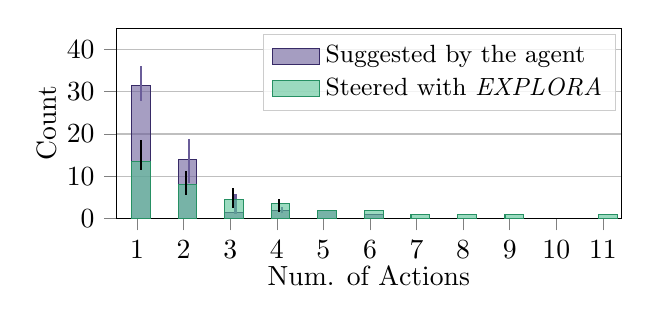
\begin{tikzpicture}
\begin{axis}[width=8cm,
height=4cm,
colormap/viridis,
ymajorgrids,
tick align=outside,
tick pos=left,
xmin=0.55, xmax=11.4,
x label style={at={(axis description cs:0.5,-0.2)},anchor=north,text depth=0pt},
y label style={at={(axis description cs:-0.1,0.5)},anchor=south,text depth=0pt},
xtick={1,...,11},
xlabel={Num. of Actions},
ylabel={Count},
ymin=0, ymax=45,
%xlabel style={font=\footnotesize},
%xticklabel style={font=\footnotesize},
%ylabel style={font=\footnotesize},
%yticklabel style={font=\footnotesize},
ytick={0,10,20,30,40},
legend cell align={left},
legend columns=1,
legend style={
	fill opacity=0.8,
	draw opacity=1,
	text opacity=1,
	at={(0.99,0.97)},
	anchor=north east,
	draw=white!80!black,
	font=\small
},
]

\draw[fill-color=150,xshift=-2pt] (axis cs:1,0) rectangle (axis cs:1.4,31.5);
\draw[draw-color=150,xshift=-2pt, thick] (axis cs:1.2,31.5) -- (axis cs:1.2, 36);
\draw[draw-color=150,xshift=-2pt, thick] (axis cs:1.2,31.5) -- (axis cs:1.2, 27.75);

\draw[fill-color=150,xshift=-2pt] (axis cs:2,0) rectangle (axis cs:2.4,14);
\draw[draw-color=150,xshift=-1.5pt, thick] (axis cs:2.2,14) -- (axis cs:2.2, 8.5);
\draw[draw-color=150,xshift=-1.5pt, thick] (axis cs:2.2,14) -- (axis cs:2.2, 18.75);

\draw[fill-color=150,xshift=-2pt] (axis cs:3,0) rectangle (axis cs:3.4,1.5);
\draw[draw-color=150,xshift=-1.5pt, thick] (axis cs:3.2,1.5) -- (axis cs:3.2, 1);
\draw[draw-color=150,xshift=-1.5pt, thick] (axis cs:3.2,1.5) -- (axis cs:3.2, 5.75);

\draw[fill-color=150,xshift=-2pt] (axis cs:4,0) rectangle (axis cs:4.4,2);
\draw[draw-color=150,xshift=-1.5pt, thick] (axis cs:4.2,2) -- (axis cs:4.2, 1.25);
\draw[draw-color=150,xshift=-1.5pt, thick] (axis cs:4.2,2) -- (axis cs:4.2, 2.75);

\draw[fill-color=150,xshift=-2pt] (axis cs:5,0) rectangle (axis cs:5.4,2);
\draw[fill-color=150,xshift=-2pt] (axis cs:6,0) rectangle (axis cs:6.4,1);


\draw[fill-color=650,xshift=-2pt] (axis cs:1,0) rectangle (axis cs:1.4,13.5);
\draw[draw,xshift=-2pt, thick] (axis cs:1.2,13.5) -- (axis cs:1.2, 18.5);
\draw[draw,xshift=-2pt, thick] (axis cs:1.2,13.5) -- (axis cs:1.2, 11.5);

\draw[fill-color=650,xshift=-2pt] (axis cs:2,0) rectangle (axis cs:2.4,8);
\draw[draw,xshift=-2.5pt, thick] (axis cs:2.2,8) -- (axis cs:2.2, 5.5);
\draw[draw,xshift=-2.5pt, thick] (axis cs:2.2,8) -- (axis cs:2.2, 11.25) ;

\draw[fill-color=650,xshift=-2pt] (axis cs:3,0) rectangle (axis cs:3.4,4.5);
\draw[draw,xshift=-2.5pt, thick] (axis cs:3.2,4.5) -- (axis cs:3.2, 2.5);
\draw[draw,xshift=-2.5pt, thick] (axis cs:3.2,4.5) -- (axis cs:3.2, 7.25);

\draw[fill-color=650,xshift=-2pt] (axis cs:4,0) rectangle (axis cs:4.4,3.5);
\draw[draw,xshift=-2.5pt, thick] (axis cs:4.2,3.5) -- (axis cs:4.2, 1.5);
\draw[draw,xshift=-2.5pt, thick] (axis cs:4.2,3.5) -- (axis cs:4.2, 4.75);

\draw[fill-color=650,xshift=-2pt] (axis cs:5,0) rectangle (axis cs:5.4,2);

\draw[fill-color=650,xshift=-2pt] (axis cs:6,0) rectangle (axis cs:6.4,2);

\draw[fill-color=650,xshift=-2pt] (axis cs:7,0) rectangle (axis cs:7.4,1);
\draw[fill-color=650,xshift=-2pt] (axis cs:8,0) rectangle (axis cs:8.4,1);
\draw[fill-color=650,xshift=-1.7pt] (axis cs:9,0) rectangle (axis cs:9.4,1);
\draw[fill-color=650,xshift=-1.5pt] (axis cs:11,0) rectangle (axis cs:11.4,1);

\addlegendimage{area legend, fill-color=150}
\addlegendimage{area legend, fill-color=650}

\legend{Suggested by the agent, Steered with \textit{EXPLORA}}
\end{axis}
\end{tikzpicture}
\end{document}